\documentclass{beamer}
\usetheme{Madrid}
\usepackage[utf8]{inputenc}
\usepackage[spanish]{babel}
\usepackage{graphicx}
\title{El Laboratorio de Investigación Industrial: Emergencia y Expansión}
\author{Por: Bruno Chaihuaque D.}
\date{}

\begin{document}
	
	\begin{frame}
		\titlepage
	\end{frame}
		% Introducción
		\begin{frame}{Inversión mundial en I+D}
			\begin{figure}
				\centering
				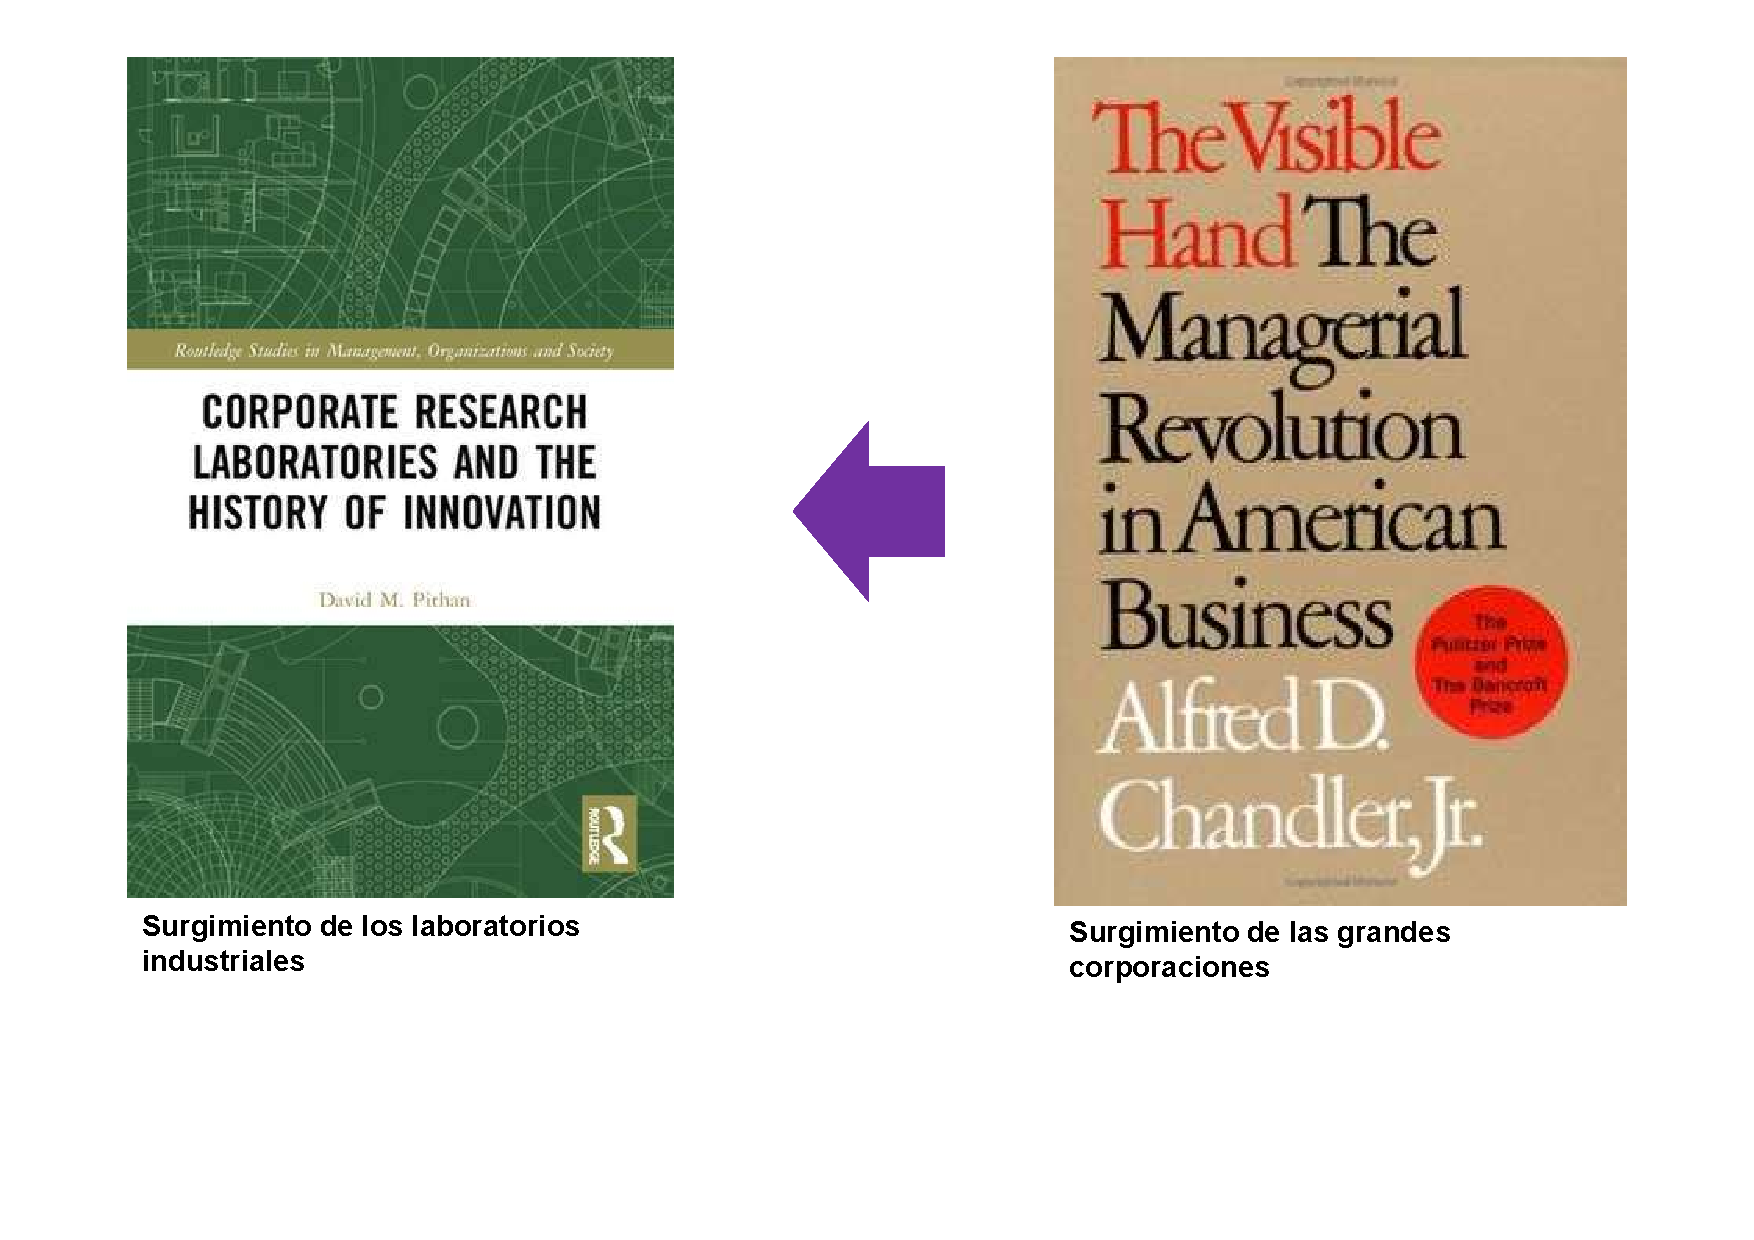
\includegraphics[width=1\linewidth]{./figs/L2.pdf}
				\caption{Inversión global en investigación y desarrollo (fuente: WIPO, 2024)}
			\end{figure}
		\end{frame}
	% Enfoque teórico
	\begin{frame}{Inversión mundial en I+D}
		\begin{figure}
			\centering
			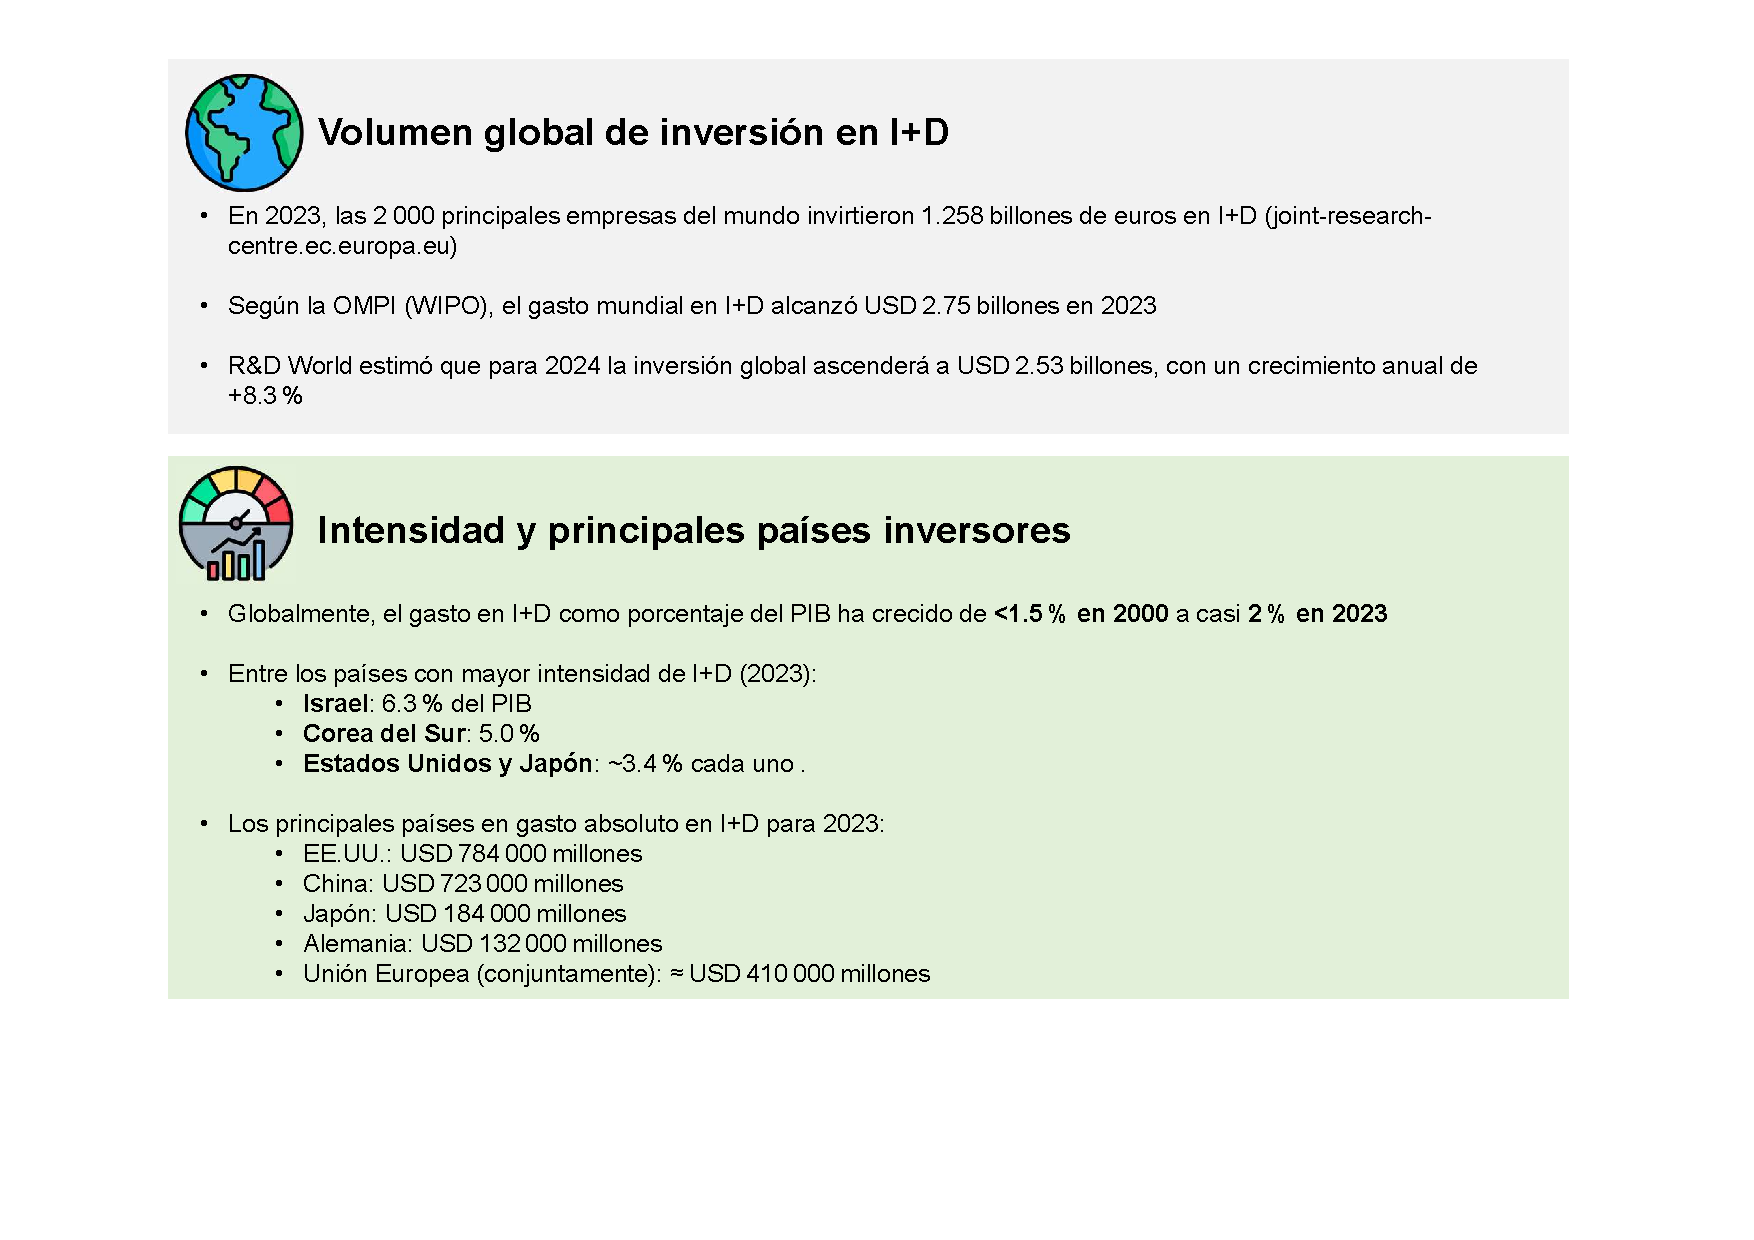
\includegraphics[width=1\linewidth]{./figs/L1.pdf}
			\caption{Inversión global en investigación y desarrollo (fuente: WIPO, 2024)}
		\end{figure}
	\end{frame}
	\begin{frame}{¿Qué enfoque teórico utiliza el texto?}
		\begin{itemize}
			\item Enfoque histórico-institucional y sociotécnico.
			\item El análisis se basa en la confluencia de:
			\begin{itemize}
				\item Transformaciones sociales: urbanización, expansión del mercado nacional y surgimiento de grandes corporaciones (Chandler, 1977).
				\item Cambios legales: Ley Antitrust Sherman (1890) y el fortalecimiento del sistema de patentes.
				\item Profesionalización científica: universidades como productores de conocimiento aplicado.
				\item Apropiación empresarial del conocimiento generado en las universidades, especialmente por científicos formados en Alemania.
			\end{itemize}
			\item Pregunta para el debate: ¿Qué relación existe entre el modelo de universidad productora de conocimiento útil y la consolidación del poder empresarial?
		\end{itemize}
	\end{frame}
	
	% Registro de datos sobre laboratorios
	\begin{frame}{¿Desde cuándo se empieza a registrar información sobre laboratorios industriales?}
		\begin{itemize}
			\item A partir de la década de 1920 se cuenta con encuestas sistemáticas sobre I+D.
			\item \textbf{Instrumentos:}
			\begin{itemize}
				\item Encuestas del \textit{National Research Council (NRC)}: 1920, 1921, 1927, 1933, 1938, 1940, 1946.
				\item Fuentes complementarias: sociedades científicas, asociaciones industriales y catálogos comerciales.
			\end{itemize}
			\item Datos recabados: número de laboratorios, tipo de investigación, disciplinas empleadas, personal científico, fecha de fundación.
			\item Problemas metodológicos: definición difusa de “investigación”, datos autorreportados sin verificación externa.
			\item Pregunta para el debate: ¿Qué desafíos presenta medir la investigación industrial desde una perspectiva cuantitativa?
		\end{itemize}
	\end{frame}
	
	% Hallazgos principales
	\begin{frame}{Principales hallazgos del capítulo}
		\begin{itemize}
			\item El laboratorio industrial surgió como respuesta organizacional a los desafíos tecnológicos y competitivos de las grandes empresas.
			\item La industria química lideró el desarrollo de laboratorios, seguida por caucho, petróleo y vidrio.
			\item Entre 1919–1928 se da la mayor expansión de laboratorios, especialmente tras la Primera Guerra Mundial.
			\item Los laboratorios permitieron:
			\begin{itemize}
				\item Internalizar la innovación.
				\item Reemplazar progresivamente al inventor independiente por el científico corporativo.
				\item Establecer estructuras permanentes de generación de conocimiento técnico.
			\end{itemize}
			\item Pregunta para el debate: ¿La consolidación de laboratorios corporativos fue un proceso democratizador del conocimiento o una forma de controlarlo?
		\end{itemize}
	\end{frame}
	
\end{document}